% Editable source for result.pdf, written by make_figures.py from run_github_39290913632/panel/result.json
\documentclass[tikz,border=6pt]{standalone}
\usepackage[T1]{fontenc}
\begin{document}
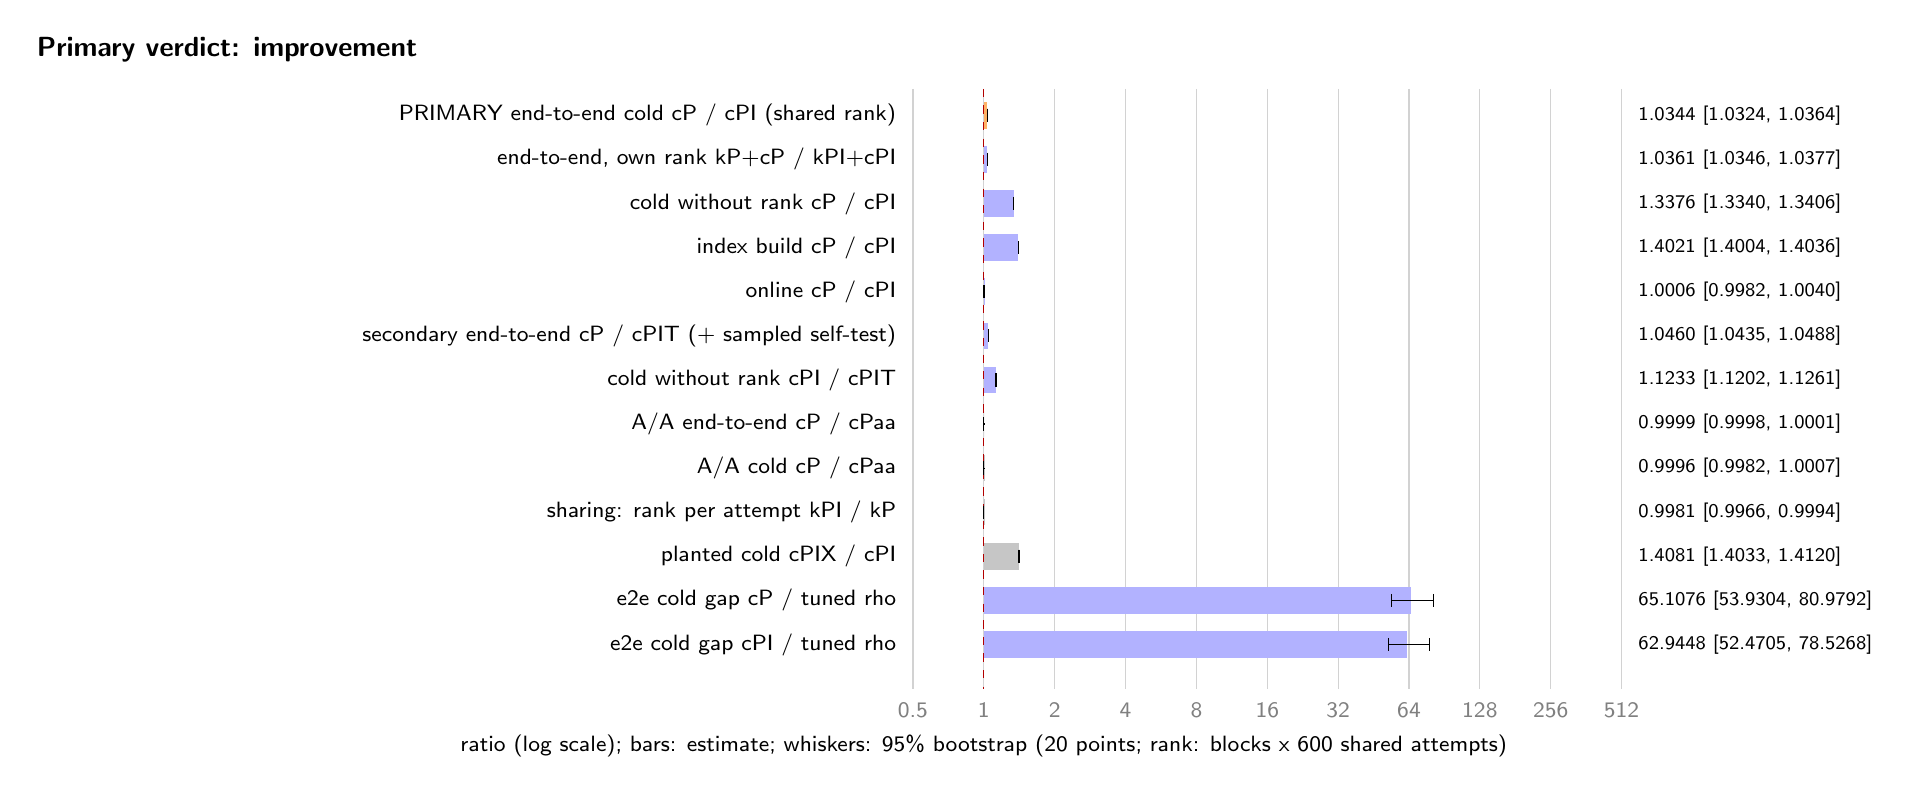
\begin{tikzpicture}[font=\sffamily\footnotesize,x=9mm,y=-5.6mm]
\draw[gray!35] (-1.0000,-0.6) -- (-1.0000,13); \node[gray] at (-1.0000,13.5) {0.5};
\draw[gray!35] (0.0000,-0.6) -- (0.0000,13); \node[gray] at (0.0000,13.5) {1};
\draw[gray!35] (1.0000,-0.6) -- (1.0000,13); \node[gray] at (1.0000,13.5) {2};
\draw[gray!35] (2.0000,-0.6) -- (2.0000,13); \node[gray] at (2.0000,13.5) {4};
\draw[gray!35] (3.0000,-0.6) -- (3.0000,13); \node[gray] at (3.0000,13.5) {8};
\draw[gray!35] (4.0000,-0.6) -- (4.0000,13); \node[gray] at (4.0000,13.5) {16};
\draw[gray!35] (5.0000,-0.6) -- (5.0000,13); \node[gray] at (5.0000,13.5) {32};
\draw[gray!35] (6.0000,-0.6) -- (6.0000,13); \node[gray] at (6.0000,13.5) {64};
\draw[gray!35] (7.0000,-0.6) -- (7.0000,13); \node[gray] at (7.0000,13.5) {128};
\draw[gray!35] (8.0000,-0.6) -- (8.0000,13); \node[gray] at (8.0000,13.5) {256};
\draw[gray!35] (9.0000,-0.6) -- (9.0000,13); \node[gray] at (9.0000,13.5) {512};
\draw[red!70!black,dashed] (0,-0.6) -- (0,13);
\node at (0,14.3) {ratio (log scale); bars: estimate; whiskers: 95\% bootstrap (20 points; rank: blocks x 600 shared attempts)};
\node[anchor=west,font=\sffamily\bfseries] at (-13.5,-1.5) {Primary verdict: improvement};
\node[anchor=east] at (-1.1000,0) {PRIMARY end-to-end cold cP / cPI (shared rank)};
\fill[orange!60] (0,-0.300000) rectangle (0.0487,0.300000);
\draw (0.0460,0) -- (0.0515,0); \draw (0.0460,-0.150000) -- (0.0460,0.150000); \draw (0.0515,-0.150000) -- (0.0515,0.150000);
\node[anchor=west,font=\sffamily\scriptsize] at (9.1000,0) {1.0344 [1.0324, 1.0364]};
\node[anchor=east] at (-1.1000,1) {end-to-end, own rank kP+cP / kPI+cPI};
\fill[blue!30] (0,0.700000) rectangle (0.0511,1.300000);
\draw (0.0491,1) -- (0.0533,1); \draw (0.0491,0.850000) -- (0.0491,1.150000); \draw (0.0533,0.850000) -- (0.0533,1.150000);
\node[anchor=west,font=\sffamily\scriptsize] at (9.1000,1) {1.0361 [1.0346, 1.0377]};
\node[anchor=east] at (-1.1000,2) {cold without rank cP / cPI};
\fill[blue!30] (0,1.700000) rectangle (0.4197,2.300000);
\draw (0.4157,2) -- (0.4229,2); \draw (0.4157,1.850000) -- (0.4157,2.150000); \draw (0.4229,1.850000) -- (0.4229,2.150000);
\node[anchor=west,font=\sffamily\scriptsize] at (9.1000,2) {1.3376 [1.3340, 1.3406]};
\node[anchor=east] at (-1.1000,3) {index build cP / cPI};
\fill[blue!30] (0,2.700000) rectangle (0.4876,3.300000);
\draw (0.4858,3) -- (0.4891,3); \draw (0.4858,2.850000) -- (0.4858,3.150000); \draw (0.4891,2.850000) -- (0.4891,3.150000);
\node[anchor=west,font=\sffamily\scriptsize] at (9.1000,3) {1.4021 [1.4004, 1.4036]};
\node[anchor=east] at (-1.1000,4) {online cP / cPI};
\fill[blue!30] (0,3.700000) rectangle (0.0009,4.300000);
\draw (-0.0025,4) -- (0.0058,4); \draw (-0.0025,3.850000) -- (-0.0025,4.150000); \draw (0.0058,3.850000) -- (0.0058,4.150000);
\node[anchor=west,font=\sffamily\scriptsize] at (9.1000,4) {1.0006 [0.9982, 1.0040]};
\node[anchor=east] at (-1.1000,5) {secondary end-to-end cP / cPIT (+ sampled self-test)};
\fill[blue!30] (0,4.700000) rectangle (0.0649,5.300000);
\draw (0.0614,5) -- (0.0688,5); \draw (0.0614,4.850000) -- (0.0614,5.150000); \draw (0.0688,4.850000) -- (0.0688,5.150000);
\node[anchor=west,font=\sffamily\scriptsize] at (9.1000,5) {1.0460 [1.0435, 1.0488]};
\node[anchor=east] at (-1.1000,6) {cold without rank cPI / cPIT};
\fill[blue!30] (0,5.700000) rectangle (0.1677,6.300000);
\draw (0.1638,6) -- (0.1713,6); \draw (0.1638,5.850000) -- (0.1638,6.150000); \draw (0.1713,5.850000) -- (0.1713,6.150000);
\node[anchor=west,font=\sffamily\scriptsize] at (9.1000,6) {1.1233 [1.1202, 1.1261]};
\node[anchor=east] at (-1.1000,7) {A/A end-to-end cP / cPaa};
\fill[gray!45] (0,6.700000) rectangle (-0.0001,7.300000);
\draw (-0.0003,7) -- (0.0001,7); \draw (-0.0003,6.850000) -- (-0.0003,7.150000); \draw (0.0001,6.850000) -- (0.0001,7.150000);
\node[anchor=west,font=\sffamily\scriptsize] at (9.1000,7) {0.9999 [0.9998, 1.0001]};
\node[anchor=east] at (-1.1000,8) {A/A cold cP / cPaa};
\fill[gray!45] (0,7.700000) rectangle (-0.0006,8.300000);
\draw (-0.0025,8) -- (0.0010,8); \draw (-0.0025,7.850000) -- (-0.0025,8.150000); \draw (0.0010,7.850000) -- (0.0010,8.150000);
\node[anchor=west,font=\sffamily\scriptsize] at (9.1000,8) {0.9996 [0.9982, 1.0007]};
\node[anchor=east] at (-1.1000,9) {sharing: rank per attempt kPI / kP};
\fill[gray!45] (0,8.700000) rectangle (-0.0027,9.300000);
\draw (-0.0049,9) -- (-0.0009,9); \draw (-0.0049,8.850000) -- (-0.0049,9.150000); \draw (-0.0009,8.850000) -- (-0.0009,9.150000);
\node[anchor=west,font=\sffamily\scriptsize] at (9.1000,9) {0.9981 [0.9966, 0.9994]};
\node[anchor=east] at (-1.1000,10) {planted cold cPIX / cPI};
\fill[gray!45] (0,9.700000) rectangle (0.4938,10.300000);
\draw (0.4889,10) -- (0.4977,10); \draw (0.4889,9.850000) -- (0.4889,10.150000); \draw (0.4977,9.850000) -- (0.4977,10.150000);
\node[anchor=west,font=\sffamily\scriptsize] at (9.1000,10) {1.4081 [1.4033, 1.4120]};
\node[anchor=east] at (-1.1000,11) {e2e cold gap cP / tuned rho};
\fill[blue!30] (0,10.700000) rectangle (6.0248,11.300000);
\draw (5.7530,11) -- (6.3395,11); \draw (5.7530,10.850000) -- (5.7530,11.150000); \draw (6.3395,10.850000) -- (6.3395,11.150000);
\node[anchor=west,font=\sffamily\scriptsize] at (9.1000,11) {65.1076 [53.9304, 80.9792]};
\node[anchor=east] at (-1.1000,12) {e2e cold gap cPI / tuned rho};
\fill[blue!30] (0,11.700000) rectangle (5.9760,12.300000);
\draw (5.7134,12) -- (6.2951,12); \draw (5.7134,11.850000) -- (5.7134,12.150000); \draw (6.2951,11.850000) -- (6.2951,12.150000);
\node[anchor=west,font=\sffamily\scriptsize] at (9.1000,12) {62.9448 [52.4705, 78.5268]};
\end{tikzpicture}
\end{document}
